157. \begin{figure}[ht!]
\center{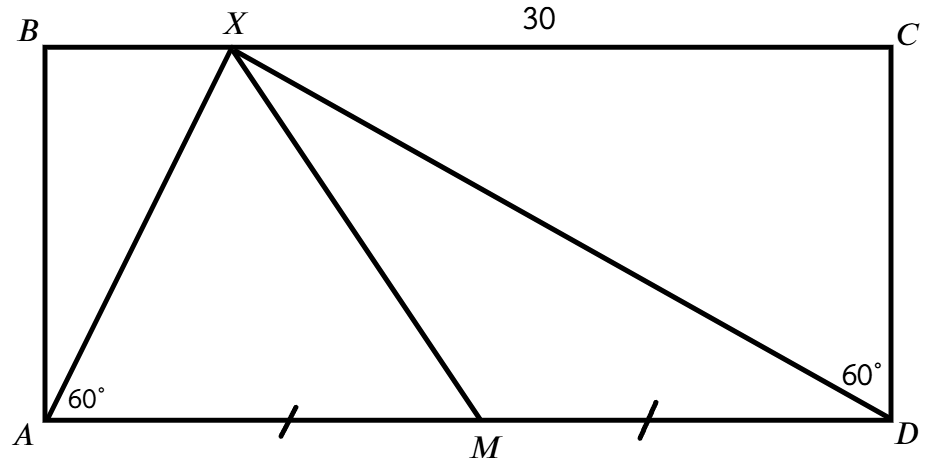
\includegraphics[scale=0.35]{g7-154.png}}
\end{figure}\\
Найдём все углы на картинке: $\angle BAX=\angle CXD=\angle ADX=90^\circ-60^\circ=30^\circ,$ тогда $\angle AXD=180^\circ-60^\circ-30^\circ=90^\circ,$ поэтому треугольник $AXD$ является прямоугольным, и его высота $XM,$ проведённая из прямого угла $AXD$ равна половине гипотенузы $AD.$ Пусть $BX=x,$ тогда по теореме о катете, лежащем напротив угла в $30^\circ,$ для треугольника $ABX$ получим соотношение $AX=2x,$ по той же теореме для треугольника $AXD$ получим равенство $AD=2\cdot2x=4x,$ поэтому $BC=BX+XC=x+30=AD=4x,$ откуда $x=10.$ Таким образом, $XM=\cfrac{1}{2}\cdot4\cdot10=20.$\\
